\section{Empirical applications and a controlled review benchmark}
\label{sec:applications}

The empirical evidence consists of two real-data applications and one
controlled synthetic benchmark. The EPA study concerns a low-cost air sensor
observed alongside a reference monitor; the VitalDB study pairs continuous
pulse oximetry with intermittent arterial-blood-gas measurements; and the AI
study pairs an automated score with expert review. These settings represent
strong local surrogacy, weaker and target-dependent surrogacy, and a controlled
local failure of an otherwise accurate surrogate. Table~\ref{tab:application-data-roles}
records how the scientific variables map to \((X,S,Y)\).

The target in each study is a local reference-outcome CDF. The analysis starts
from complete paired outcomes and then reveals \(Y\) under
known reference-sampling probabilities while retaining \((X,S)\) for every
unit. For EPA and VitalDB, the benchmark \(F_{h,\mathrm{emp}}\) is the
kernel-localized empirical CDF computed from all available reference outcomes.
The synthetic AI benchmark instead uses the population target \(F_{h,0}\).
Repeated reference sampling measures recovery of these study-specific local
distributions.

\begin{table}[!t]
\centering
\small
\setlength{\tabcolsep}{4pt}
\renewcommand{\arraystretch}{1.15}
\caption{Data structure and inferential role of the empirical studies.}
\label{tab:application-data-roles}
\begin{tabular}{@{}>{\RaggedRight\arraybackslash}p{0.12\textwidth}>{\RaggedRight\arraybackslash}p{0.17\textwidth}>{\RaggedRight\arraybackslash}p{0.24\textwidth}>{\RaggedRight\arraybackslash}p{0.18\textwidth}>{\RaggedRight\arraybackslash}p{0.22\textwidth}@{}}
\toprule
Study & Analysis units & Reference outcome and surrogate & Localization & Distributional question \\
\midrule
EPA air sensors
& 2,814 collocated site-days at seven U.S. sites
& Reference-monitor PM$_{2.5}$; uncorrected PurpleAir PM$_{2.5}$
& Relative humidity at 30\%, 50\%, and 70\%
& Recovery of humidity-specific PM$_{2.5}$ distributions and upper-tail quantiles from sparse reference monitoring \\
VitalDB oximetry
& 3,178 subjects with one matched measurement pair each
& Arterial-blood-gas SaO$_2$; pulse-oximeter SpO$_2$
& Elapsed case time at 30, 75, and 180 minutes
& Recovery of a discrete saturation distribution when the continuous surrogate becomes less informative locally \\
AI-assisted review
& 2,998 evaluated dossiers in a controlled synthetic corpus
& Mean of three expert ratings; automated score
& Standardized complexity at $x_0=0$
& Recovery of expert-score distributions under scarce or selective review, including controlled local surrogate reversal \\
\bottomrule
\end{tabular}
\end{table}


\begin{table}[!t]
\centering
\footnotesize
\setlength{\tabcolsep}{2.5pt}
\caption{Primary results under controlled reference sampling. EPA and VitalDB use their localized complete-data empirical benchmarks; AI uses its population benchmark.}
\label{tab:application-primary}
\begin{tabular}{llrrrrrl}
\toprule
Study & Target & Ref. frac. & Anchor & Full & Adaptive & Mean wt. & Adaptive/Anchor [95\% MC] \\
\midrule
EPA & 30\% RH & 10.0\% & 2.060 & 0.738 & 0.818 & 0.846 & 0.397 [0.337, 0.457] \\
 & 50\% RH & 10.0\% & 0.864 & 0.375 & 0.386 & 0.888 & 0.447 [0.385, 0.510] \\
 & 70\% RH & 10.0\% & 1.601 & 0.722 & 0.765 & 0.862 & 0.478 [0.423, 0.534] \\
VitalDB & 30 min & 10.0\% & 0.205 & 0.177 & 0.181 & 0.803 & 0.882 [0.851, 0.914] \\
 & 75 min & 10.0\% & 0.393 & 0.347 & 0.349 & 0.867 & 0.888 [0.857, 0.919] \\
 & 180 min & 10.0\% & 0.241 & 0.232 & 0.234 & 0.672 & 0.971 [0.949, 0.992] \\
AI & Random review & 2.5\% & 9.091 & 3.380 & 4.195 & 0.775 & 0.461 [0.427, 0.496] \\
 & Random review & 10.0\% & 2.147 & 0.814 & 0.861 & 0.891 & 0.401 [0.363, 0.439] \\
 & Random review & 40.0\% & 0.434 & 0.197 & 0.199 & 0.955 & 0.457 [0.421, 0.494] \\
\bottomrule
\end{tabular}
\vspace{2pt}
\parbox{0.98\textwidth}{\footnotesize ISE values are multiplied by $10^3$. Risk-ratio intervals use common reference samples and quantify Monte Carlo variation conditional on the stated study-specific benchmark; they are not population-sampling confidence intervals.}
\end{table}


\subsection{Air-quality distributions at fixed humidity}

Dense low-cost sensor networks can provide much broader coverage than
regulatory or research-grade monitors, but the field relationship between the
two instruments changes with environmental conditions. Humidity is especially
relevant to particle-sensor response. The resulting question is distributional:
at a specified humidity, how much mass and upper-tail probability would the
reference monitor assign to different PM\(_{2.5}\) levels? A correction aimed
only at the conditional mean does not determine that local distribution.

We use the public EPA long-term air-sensor study, in which six commercial sensor
types were collocated with reference monitors at seven U.S. sites in 2019--2021
\citep{barkjohn2025sensors,epa2025longtermdata}. Uncorrected PurpleAir hourly
measurements are aggregated to 2,814 site-days. Set
\(Y=\log(1+\text{reference PM}_{2.5})\),
\(S=\log(1+\text{PurpleAir PM}_{2.5})\), and \(X\) to relative humidity; the
targets are 30\%, 50\%, and 70\%. PurpleAir is an imperfect surrogate; the
complete collocations define the reference distribution.

Random reference sampling and sampling selective on sensor level and humidity
are examined at 5\%, 10\%, and 20\% budgets. Calendar weeks, rather than
individual site-days, are assigned to fitting, weight selection, and CDF
evaluation, preserving the temporal grouping in the collocation study. Each
design--budget--target combination is evaluated over 500 reference-sampling
repetitions, with the same reference sample used for all methods.

\begin{figure}[!t]
\centering
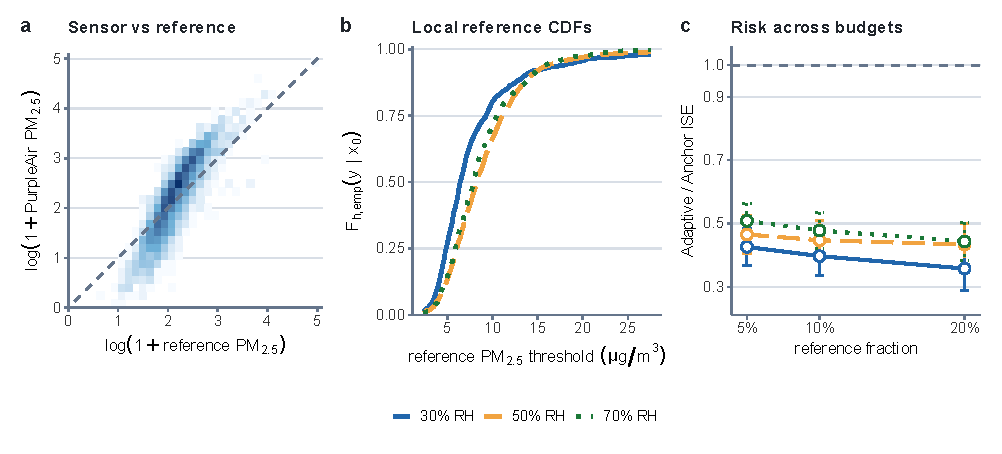
\includegraphics[width=\textwidth]{figures/figure4_epa_application.pdf}
\caption{EPA long-term air-sensor application. Panel (a) displays all 2,814
collocated site-days on the log scale; darker bins contain more observations
and the dashed line is equality between the PurpleAir and reference-monitor
measurements. Panel (b) shows the complete-data kernel-localized empirical CDF
at 30\%, 50\%, and 70\% relative humidity, using a bandwidth of
ten humidity percentage points. Panel (c) reports Adaptive-to-Anchor mean ISE
ratios under 5\%, 10\%, and 20\% random reference sampling. Vertical ranges are
paired 95\% Monte Carlo intervals from 500 reference-sampling repetitions; the horizontal line at
one is the Anchor risk.}
\label{fig:epa-application}
\end{figure}

Figure~\ref{fig:epa-application}(a) shows a strong overall sensor--reference
relationship together with appreciable spread around equality. The
complete-data local CDFs in panel (b) also change across humidity targets; the
30\% curve places more mass at lower PM\(_{2.5}\) thresholds than the 50\% and
70\% curves. Thus the application involves both calibration error and a target
distribution that varies with the localization variable.

% CLAIM_READY: APP-EPA
At the 10\% random-reference budget in
Table~\ref{tab:application-primary}, Adaptive reduces mean ISE by 52.2--60.3\%
across the humidity targets, with the largest gain at 30\%. All three paired
Monte Carlo intervals for the risk ratio exclude one, and mean borrowing
remains between 0.846 and 0.888. Full has lower mean ISE at all three targets,
with paired intervals also favoring Full. Adaptive's observed
negative-transfer frequency ranges from 9.0\% to 13.6\%, compared with
10.0--15.8\% for Full; the largest separation occurs at 50\% humidity.

Panel (c) extends that comparison over all nine random-sampling cells.
Adaptive-to-Anchor risk ratios range from 0.358 to 0.508, and every paired
interval lies below one. The gain is largest near 30\% humidity but remains
substantial throughout the humidity and reference-budget ranges.

The gain extends to the upper tail: the conditional 0.90-quantile error is
lower at every humidity target. At 30\% humidity, Adaptive reduces mean
absolute error from 2.00 to 0.83 micrograms per cubic meter; the reductions at
50\% and 70\% have the same direction. For the fixed reference sample, weekly
cluster-multiplier bands are 19--30\% narrower than the anchor bands and
contain the complete-data CDF at all three targets.

\subsection{Oxygen-saturation distributions during surgery}

Pulse oximetry supplies a continuous, noninvasive oxygen-saturation signal,
whereas arterial-blood-gas analysis supplies a more direct but intermittent
reference measurement. Their relationship need not be constant over a
surgical case. Moreover, the lower tail of the SaO\(_2\) distribution carries
information that is not summarized by a mean calibration equation, while the
upper end is strongly discrete: saturation values are bounded and often
recorded at 100.

VitalDB combines high-resolution intraoperative monitoring with laboratory
measurements \citep{lee2022vitaldb}. We match each arterial SaO\(_2\)
measurement to the nearest pulse-oximeter SpO\(_2\) reading from the same case
within one second. An analysis-independent rule selects one pair per subject,
leaving 3,178 independent subject-level records from 8,476 eligible pairs.
Here \(Y\) is SaO\(_2\), \(S\) is SpO\(_2\), and
\(X=\log(1+\text{elapsed case time})\). The local targets are 30, 75, and 180
minutes.

Random sampling and sampling favoring low SpO\(_2\) values retain 5\%, 10\%,
20\%, or 40\% of arterial measurements as reference outcomes. Each
design--budget combination is evaluated over 500 sampling repetitions; the
reference samples are nested across budgets and shared across targets.

\begin{figure}[!t]
\centering
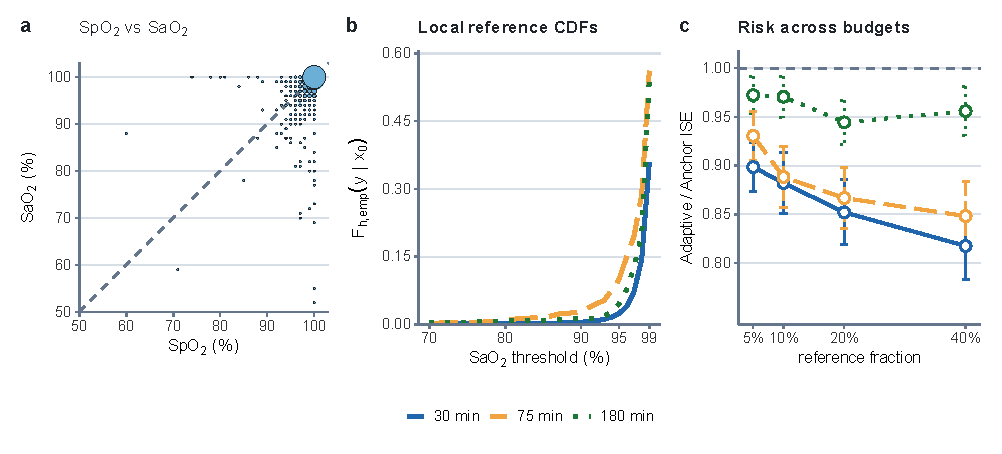
\includegraphics[width=\textwidth]{figures/figure5_vitaldb_application.pdf}
\caption{VitalDB oxygen-saturation application. Panel (a) displays all 3,178
subject-level SaO\(_2\)--SpO\(_2\) pairs; point area is proportional to the
number of observations at each integer pair and the dashed line is equality.
Panel (b) shows the complete-data kernel-localized empirical SaO\(_2\) CDF at
30, 75, and 180 minutes on the threshold grid from 70 through 99.
Panel (c) reports Adaptive-to-Anchor mean ISE ratios under 5\%, 10\%, 20\%, and
40\% random reference sampling. Vertical ranges are paired 95\% Monte Carlo
intervals from 500 reference-sampling repetitions; the horizontal line at one is the Anchor
risk.}
\label{fig:vitaldb-application}
\end{figure}

Figure~\ref{fig:vitaldb-application}(a) displays the discreteness of both
measurements and the concentration near the upper boundary. In the primary
sample, 52.3\% of SaO\(_2\) values equal 100. Panel (b) shows that the local
reference CDF also changes with elapsed time, particularly over the upper
jumps represented on the threshold grid.

% CLAIM_READY: APP-VITALDB
At the 10\% random budget, Adaptive lowers mean ISE by 11.8\%, 11.2\%, and
2.95\% at the three successive target times. All three paired
anchor-minus-Adaptive intervals exclude zero. Full has lower mean ISE; its
paired advantage over Adaptive is conclusive at 30 minutes but not at the two
later targets.

The risk ratio reaches 0.971 at 180 minutes, and mean borrowing falls to 0.672
there from 0.803--0.867 at the earlier targets. Panel (c) shows the same
ordering over the full budget grid: the largest gain occurs at 30 minutes,
whereas the 180-minute ratios remain closest to one.

Adaptive's observed negative-transfer frequency is 1.2--4.4 percentage points
lower than Full's; the paired frequency contrast excludes zero at 75 and 180
minutes. Adaptive nevertheless exceeds anchor risk in 35.4--46.8\% of sampling repetitions,
a larger frequency than in the EPA and aligned AI studies.

The target-specific loss of surrogate information is also present in the
paired data. Local SpO\(_2\)--SaO\(_2\) correlations are 0.498, 0.465, and
0.213 at the three target times. The 30-minute neighborhood contains only
three values below 90, and the lower tail remains sparse at the later targets.
The weaker 180-minute association and small lower-tail counts leave less scope
for a surrogate correction even though the overall reference budget is
unchanged.

Within the evaluated grid, the information multiplier for a 10\% Adaptive
budget decreases from 1.109 at 30 minutes to 1.027 at 180 minutes, mirroring
the decline in local surrogate association.

\subsection{Controlled benchmark for limited expert review}

The third study is a controlled synthetic benchmark rather than an external
data application. Automated assessment provides a broadly available surrogate,
whereas panel review is costly enough to be collected only for a subset of
cases. The target is the distribution of expert-panel scores at a fixed level
of dossier complexity. This construction permits the review law and local
surrogate error to be varied while retaining a known population benchmark---a
combination unavailable in the two observational applications.

Here \(X\) is standardized complexity, \(S\) is the automated score,
and \(Y\) is the mean of three expert ratings. The primary target is
\(x_0=0\), the center of the complexity scale. In confidence-triggered review
designs, the broadly observed model-confidence score \(C\) also enters the
known verification law through \(W=(X,S,C)\); the augmentation candidates use
\((X,S)\).

Synthetic dossiers contain performance dimensions, verified adverse events,
operating complexity, and contextual information, but exclude the panel score
and latent generating variables. Three independent corpora contain 3,000,
1,500, and 1,500 dossiers. Each dossier was scored under a common rubric before
any expert-review samples were drawn; 5,997 of 6,000 evaluations yielded valid
scores. Corpus A is used for the primary analysis, and a second automated
evaluator provides a sensitivity analysis. The complete scoring specifications
and prompts are reported in the Supplement.

\begin{figure}[H]
\centering
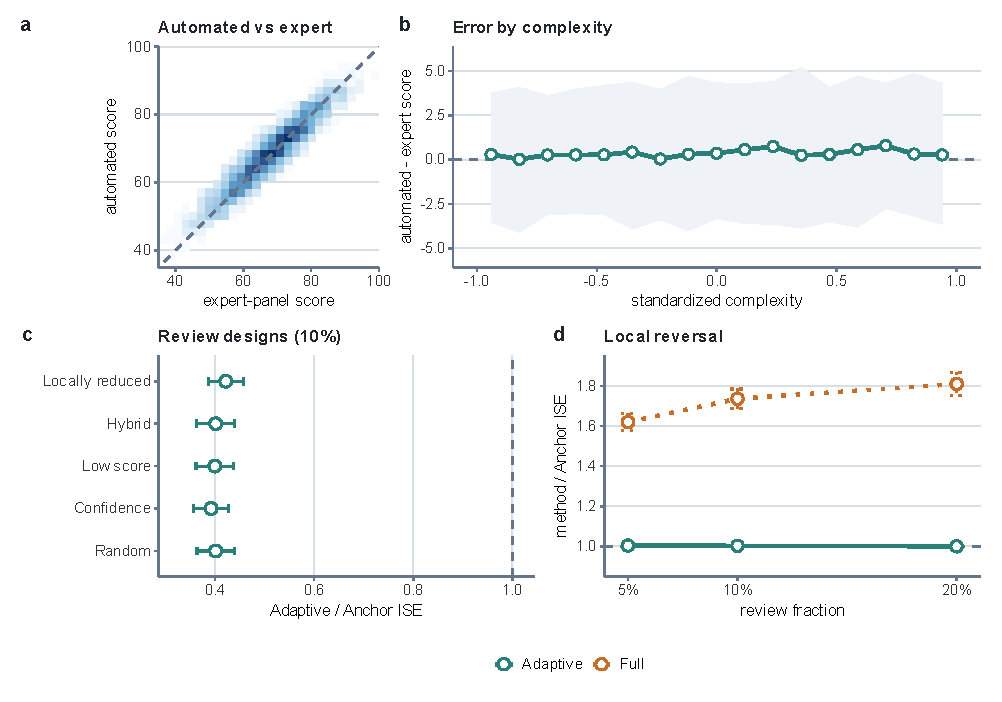
\includegraphics[width=\textwidth]{figures/figure6_ai_review.pdf}
\caption{Controlled synthetic AI-assisted review benchmark. The risk benchmark
is the population localized expert-score CDF at \(x_0=0\). Panel (a) displays
all 2,998 valid automated scores against corrected expert-panel scores;
darker bins contain more dossiers and the dashed line is equality. Panel (b)
reports mean automated-minus-expert score in 17 fixed complexity bins; the
pale envelope spans the empirical 10th and 90th score-error percentiles within
each bin. Panel (c) reports Adaptive-to-Anchor mean ISE ratios for five review
designs at a 10\% review fraction. Panel (d) reports Adaptive- and
Full-to-Anchor mean ISE ratios under locally reduced review and local surrogate
reversal. Intervals in panels (c)--(d) are paired 95\% Monte Carlo intervals
from 2,000 sampling repetitions; the horizontal line at one is the Anchor risk.}
\label{fig:ai-review}
\end{figure}

Each review design is evaluated over 2,000 sampling repetitions. The designs
include random review, confidence- or score-triggered review, a hybrid rule,
and reduced review near \(x_0=0\). Each design is calibrated to its stated mean
review fraction.

% CLAIM_READY: APP-AI-REFERENCE
On the 2,998 valid Corpus-A cases, the AI score has mean absolute error 2.415
and Pearson correlation 0.946 with the corrected expert outcome; the
calibration slope is 0.992. The maximum absolute local bias over the analysis
bins is 0.782. Reported confidence has correlation 0.159 with negative absolute
error. High global score correlation therefore coexists with local bias and a
weak confidence-based review signal.

The overall score relation in Figure~\ref{fig:ai-review}(a) is strong, but
panel (b) shows that automated-minus-expert error still varies across local
complexity bins. This separates global predictive accuracy from the local
distributional relation on which borrowing at \(x_0\) depends.

% CLAIM_READY: APP-AI-DOWNSTREAM
Under random review, Adaptive reduces mean ISE by 53.9--59.9\% over reference
fractions 0.025--0.40. Its mean borrowing weight increases from 0.775 to 0.955,
while the Adaptive-to-anchor risk ratio remains between 0.401 and 0.461. Full
has lower mean ISE at every fraction, although the absolute Full--Adaptive gap
contracts as the review fraction increases. For fractions up to 0.10, the
anchor requires 2.28--2.50 times the actual random-review fraction to match
Adaptive risk within the evaluated grid.

% CLAIM_READY: APP-AI-CONTROLLED
Across the five primary review designs, Adaptive gains range from 35.8\% to
61.1\%. Confidence-triggered review closely follows random review, consistent
with the weak confidence--error association. Reduced review near \(x_0\) has
the smallest gain at the lowest review budget; the selection and evaluation
folds then contain fewer local reference observations. At the 10\% budget,
the five Adaptive-to-Anchor ratios in Figure~\ref{fig:ai-review}(c) lie between
0.392 and 0.422.

With locally reduced review and surrogate reversal, the mean weight falls from
0.072 to 0.001 as \(p\) rises from 0.05 to 0.20; mean losses are 0.39\%, 0.27\%,
and approximately zero. Full's negative-transfer frequency is 75.3--79.4\%.

% CLAIM_READY: APP-AI-BANDS
In six representative AI band settings, Adaptive simultaneous coverage is
0.940--0.974. Its integrated bands are 6.8--29.7\% narrower than anchor bands
in every setting. Reduced local review produces the widest bands and the lowest
Adaptive coverage, whereas the aligned random and hybrid designs retain the
largest width reductions.

\subsection{Comparison across the studies}

% CLAIM_READY: APP-SYNTHESIS
Across the examined budget grids, Adaptive-to-anchor risk ratios are
0.358--0.508 for EPA, 0.401--0.461 for random AI review, and 0.818--0.972 for
VitalDB. Every paired interval remains below one, but the size of the gain is
target specific. EPA and the aligned AI design combine high borrowing with
large risk reductions. VitalDB yields smaller gains, especially at 180 minutes
where the local SpO\(_2\)--SaO\(_2\) relation is weakest.

Full often has slightly lower mean risk in the aligned settings. That ordering
reflects the cost of estimating a weight on a separate fold when the best path
is close to full borrowing. The comparison changes under local reversal:
Adaptive selects weights near zero and sharply lowers the observed
negative-transfer frequency relative to Full. Across the three studies, the
selected weight follows local distributional alignment more closely than any
single global measure of surrogate accuracy.
